% Gemini theme
% https://github.com/anishathalye/gemini
%
% We try to keep this Overleaf template in sync with the canonical source on
% GitHub, but it's recommended that you obtain the template directly from
% GitHub to ensure that you are using the latest version.

\documentclass[final]{beamer}

% ====================
% Packages
% ====================

\usepackage[T1]{fontenc}
\usepackage{lmodern}
\usepackage[size=a0,scale=1.25]{beamerposter}
\usetheme{gemini}
\usecolortheme{amii}
\usepackage{graphicx}
\usepackage{booktabs}
\usepackage{tikz}
\usepackage{pgfplots}
\usepackage{subfigure}

% ====================
% Lengths
% ====================

% If you have N columns, choose \sepwidth and \colwidth such that
% (N+1)*\sepwidth + N*\colwidth = \paperwidth
\newlength{\sepwidth}
\newlength{\colwidth}
\setlength{\sepwidth}{0.025\paperwidth}
\setlength{\colwidth}{0.3\paperwidth}

\newcommand{\separatorcolumn}{\begin{column}{\sepwidth}\end{column}}

% ====================
% Title
% ====================

\title{\LARGE{Comparing Direct and Indirect Temporal-Difference Methods for Estimating the Variance of the Return}}

\author{Craig Sherstan, Dylan R. Ashley$^{*}$, Brendan Bennett$^{*}$, Kenny Young, Adam White, Martha White, Richard S. Sutton}

\institute[shortinst]{Reinforcement Learning and Artificial Intelligence Laboratory, University of Alberta}

% ====================
% Body
% ====================

\begin{document}

\begin{frame}[t]
\begin{columns}[t]
\separatorcolumn

\begin{column}{\colwidth}

    \begin{block}{Background}
        In a Markov Decision Process the return is defined to be the discounted sum of future rewards:
        \begin{equation*}
            G_{\,t} = R_{\,t + 1} + \gamma_{\,t + 1} \,R_{\,t + 2} + \gamma_{\,t + 1} \,\gamma_{\,t + 2} \,R_{\,t + 3} + \ldots
        \end{equation*}
        The {$\lambda$}-return provides a bias-variance trade-off controlled by a new hyperparameter $\lambda$ and often is easier to learn while being just as useful (we use $J$ to denote the expected value of the return from a state, or the \textit{value} of a state):
        \begin{equation*}
            G_{\,t}^{\,\lambda} = R_{\,t+1} + \gamma_{\,t + 1} \,(1 - \lambda_{\,t + 1}) \,J_{\,t}(S_{\,t + 1}) + \gamma_{\,t + 1} \,\lambda_{\,t + 1} \,G^{\,\lambda}_{\,t + 1}
        \end{equation*}
        Note that the {$\lambda$}-return is exactly equal to the return when $\lambda$ is kept at $1$.
    \end{block}

    \begin{block}{Motivation}
        We might want to learn the variance of the return as
        \begin{itemize}
            \item it lets us take risk into account when making decisions \cite{tamar2016learning},
            \item we can use it for hyperparameter tuning \cite{white2016greedy},
            \item we can use it to guide exploration \cite{white2014surprise}, and
            \item we can use it to improve our representation \cite{ring1997child}.
        \end{itemize}
    \end{block}

    \begin{alertblock}{Direct Method}
        We present a new, direct approach \cite{sherstan2018comparing} that works by learning the expected value and variance of the return using TD($\lambda$). The direct method uses the following variance estimator:
        \begin{align*}
            \bar{\gamma}_{\,t + 1} &\leftarrow \gamma_{\,t + 1}^{\,2} \\
            \bar{R}_{\,t + 1} &\leftarrow \delta_{\,t}^{\,2} \\
            \bar{\delta}_{\,t} &\leftarrow \bar{R}_{\,t + 1} + \bar{\gamma}_{\,t + 1} \,J_{\,t}(s') - J_{\,t}(s) \\
            V_{\,t + 1}(s) &\leftarrow V_{\,t}(s) + \bar{\alpha} \,\bar{\delta}_{\,t}
        \end{align*}
        Both the direct and the existing indirect method \cite{white2016greedy} can be viewed as a network of learners:
        \begin{figure}
            \centering
            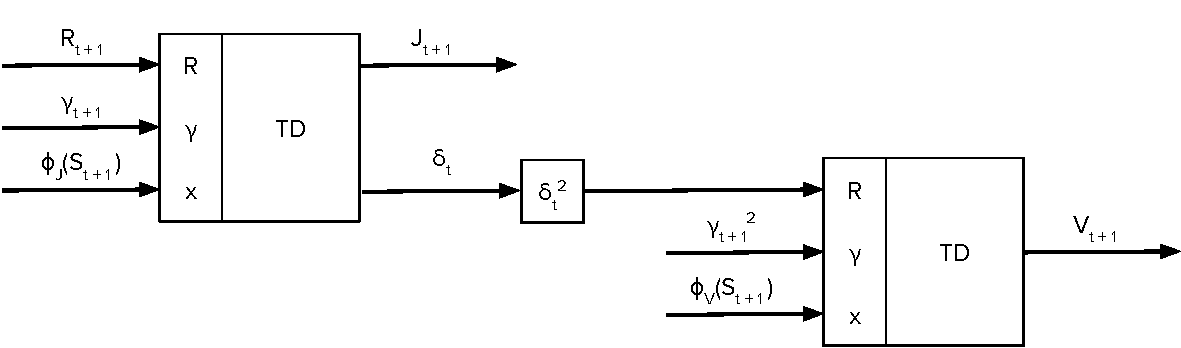
\includegraphics[height=7.5cm]{{images/direct.pdf}}
            \caption{The direct method}
        \end{figure}
        \begin{figure}
            \centering
            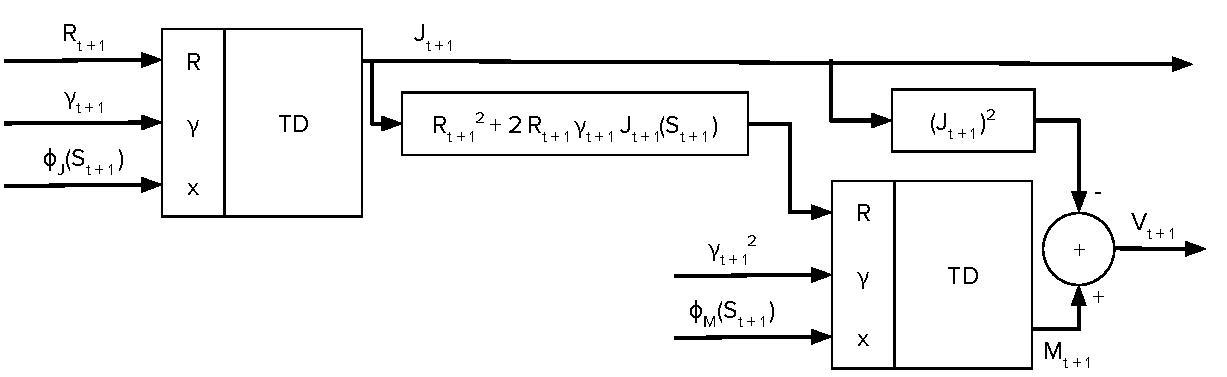
\includegraphics[height=8.25cm]{{images/indirect.pdf}}
            \caption{The indirect method}
        \end{figure}
    \end{alertblock}

\end{column}

\separatorcolumn

\begin{column}{\colwidth}
    \begin{block}{Intuition}
        For a random variable $X$, the variance of $X$ can be expressed as \(\mathbb{E}[(X - \mathbb{E}[X])^{\,2}]\). Similarly, the variance of the {$\lambda$}-return can be expressed in terms of temporal difference (TD) errors:
        \vspace{0.1em}
        \begin{equation*}
            \big(G_{\,t}^{\,\lambda} - J(S_{\,t})\big)^{\,2}
                = \bigg(\sum_{n = 0}^{\infty} \delta_{\,t + n} \prod_{k = 1}^{n} \gamma_{\,t + k} \,\lambda_{\,t + k}\bigg)^{\,2}
                \approx \sum_{n = 0}^{\infty} \delta_{\,t + n}^{\,2} \prod_{k = 1}^{n} \gamma_{\,t + k}^{\,2} \,\lambda_{\,t + k}^{\,2}
            \vspace{0.3em}
        \end{equation*}
        This has the form of a Bellman equation:
        \begin{equation*}
            \mathrm{Var}[G_{\,t}^{\,\lambda}]
                \approx V(S_{\,t})
                = \mathbb{E}[\delta_{\,t}^{\,2} + \gamma_{\,t + 1}^{\,2} \,\lambda_{\,t + 1}^{\,2} \,V(S_{\,t + 1})]
        \end{equation*}
        and so can be approximated using temporal difference methods.
    \end{block}

    \begin{block}{Tabular Results}
        We compare both methods on a chain domain first:
        \begin{figure}
            \centering
            \includegraphics[height=4cm]{{images/chain/state_diagram.pdf}}
        \end{figure}
        For this domain we highlight the resilience our method to differences in step sizes between the value and variance learners:
        \begin{figure}
            \centering
            \subfigure[]{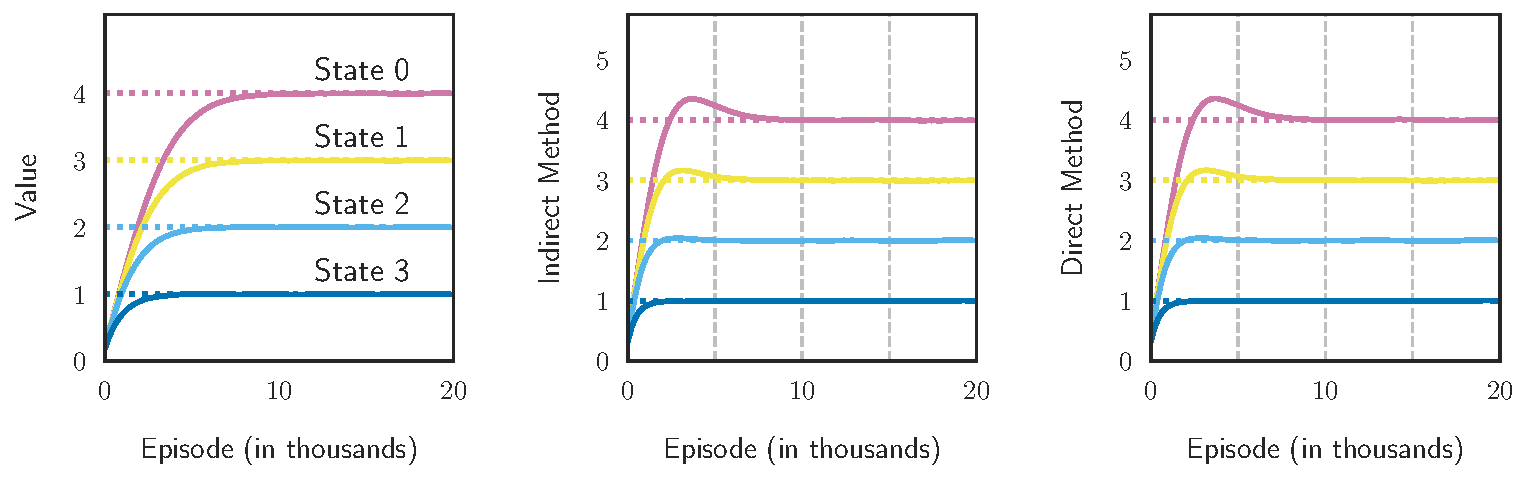
\includegraphics[height=8.5cm]{images/chain/same_step_size.pdf}}
            \vspace{0.5em}
            \subfigure[]{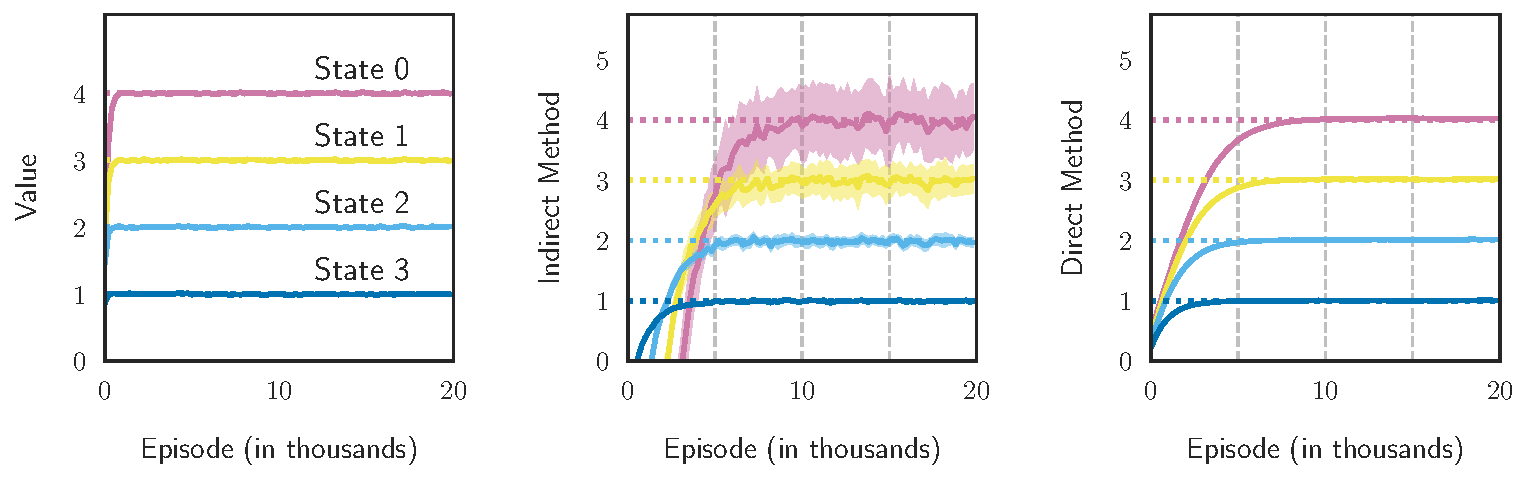
\includegraphics[height=8.5cm]{images/chain/value_step_size_greater.pdf}}
            \vspace{0.5em}
            \subfigure[]{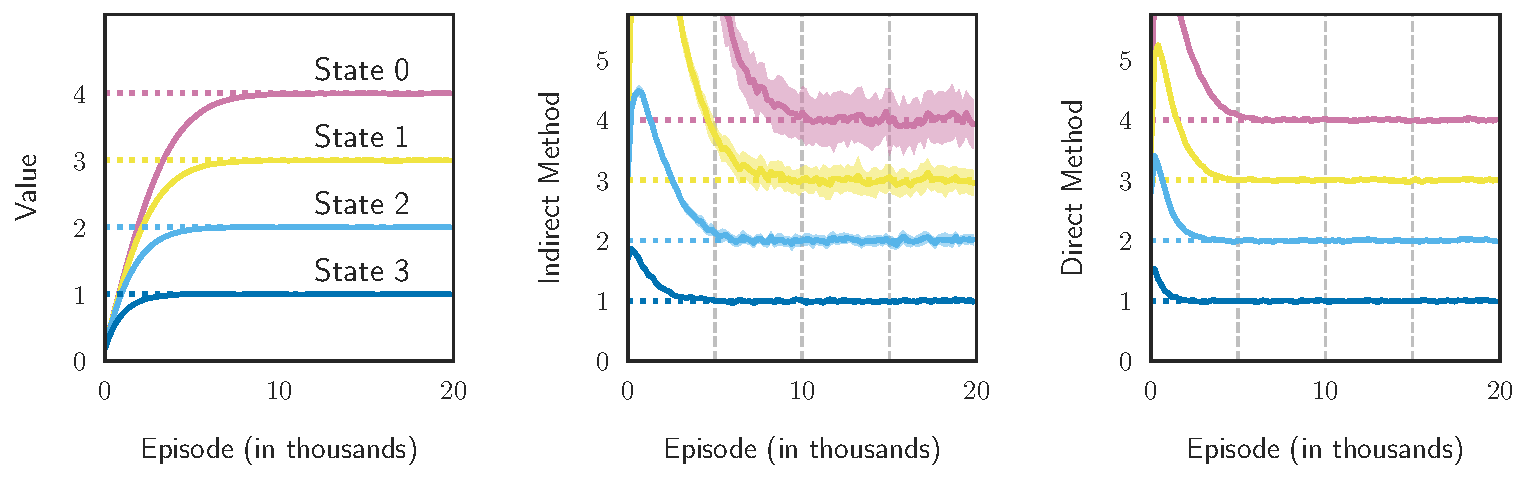
\includegraphics[height=8.5cm]{images/chain/variance_step_size_greater.pdf}}
            \caption{Learning on chain with \textbf{a)} step-sizes equal ($\alpha = \bar{\alpha} = 0.001$), \textbf{b)} value step-size larger, ($\alpha = 0.01, \bar{\alpha} = 0.001$), \textbf{c)} variance step-size larger, ($\alpha = 0.001, \bar{\alpha} = 0.01$)}
        \end{figure}
    \end{block}

    \begin{figure}
        \centering
        \vspace{-0.625cm}
        \hspace{-0.625cm}
        
\includegraphics[height=3cm]{{images/logos/ualberta.png}}
        \hspace{5cm}
        
\includegraphics[height=4cm]{{images/logos/amii.png}}
        \hspace{6.25cm}
        
\includegraphics[height=4cm]{{images/logos/rlai.png}}
    \end{figure}

\end{column}

\separatorcolumn

\begin{column}{\colwidth}

    \begin{block}{Linear Function Approximation Results}
        We experiment on a function approximation scheme overlaying a tabular random walk:
        \begin{figure}
            \centering
            \vspace{-1em}
            \includegraphics[height=5cm]{{images/random_walk/state_diagram.pdf}}
            \vspace{-1em}
        \end{figure}
        For state $S_{\,i}$ the value estimator uses \(\phi_{\,t} = [1, i]\) and the variance estimator uses \(\phi_{\,t} = [1, i, i^2]\). Here we highlight the faster learning and better convergence of our method:
        \begin{figure}
            \centering
            \vspace{-1em}
            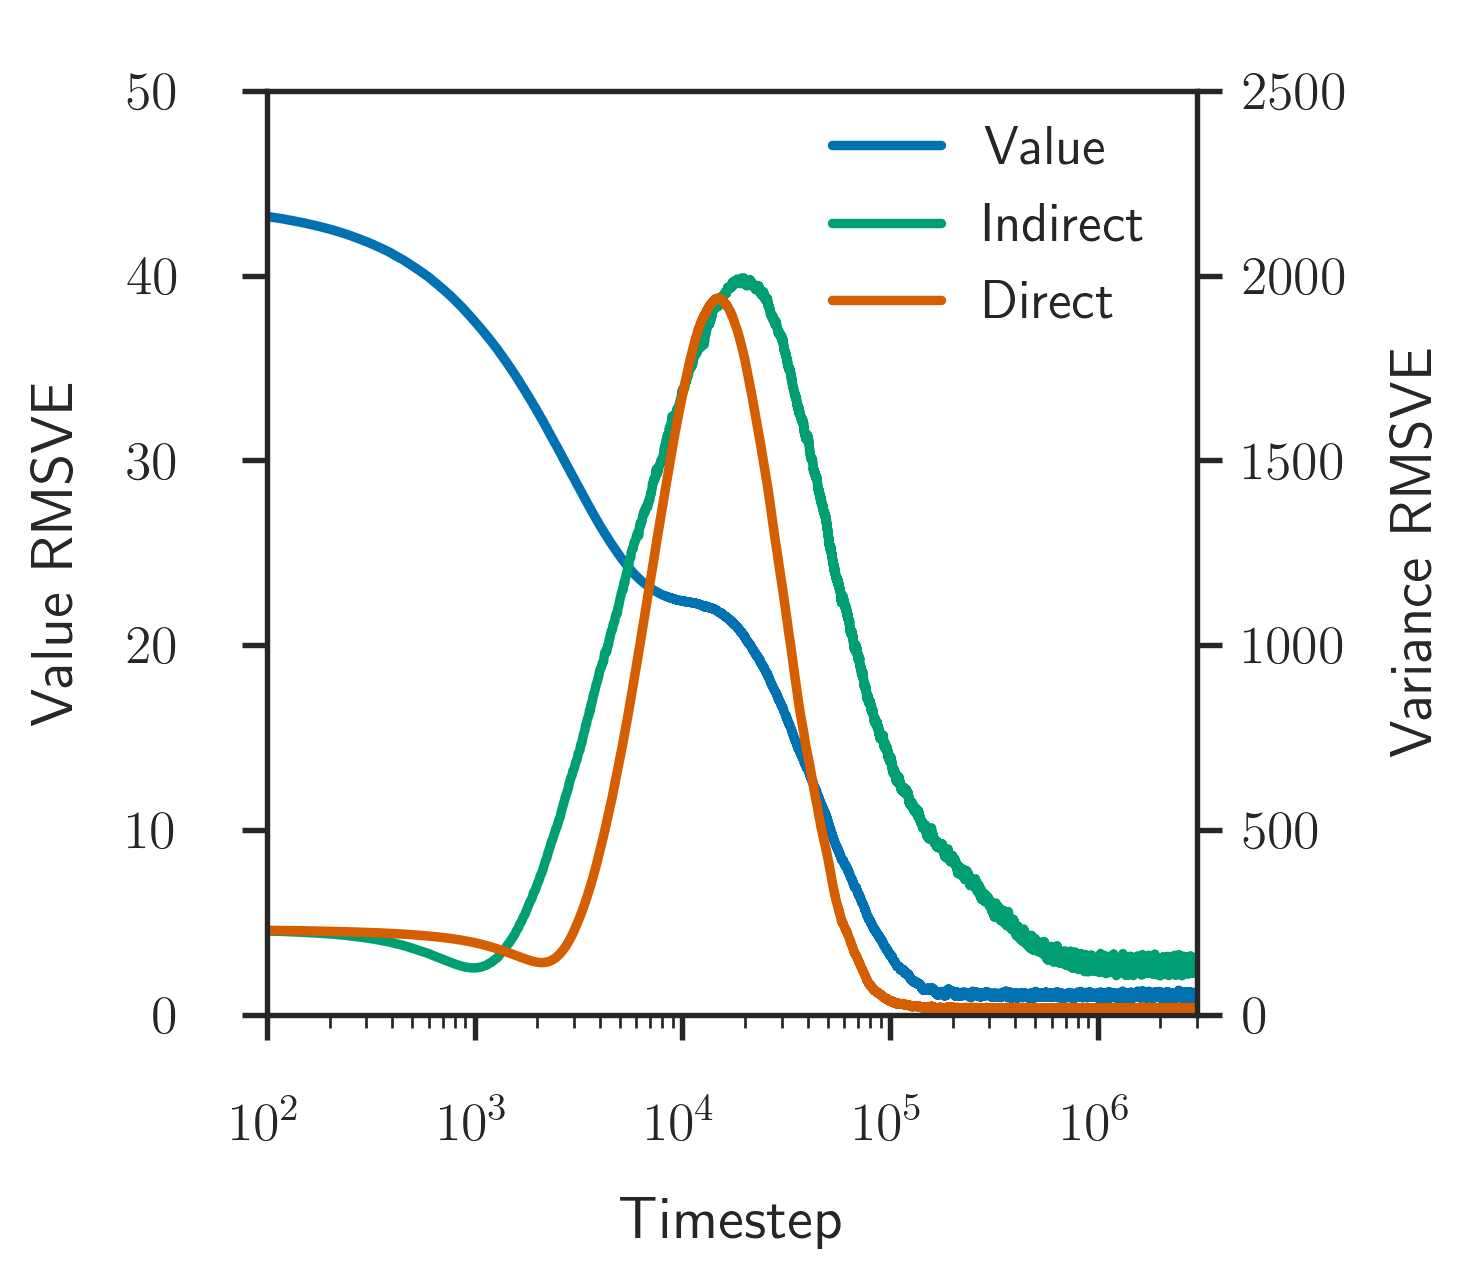
\includegraphics[height=13cm]{{images/random_walk/performance.png}}
        \end{figure}
    \end{block}

    \begin{alertblock}{Conclusions}
        In general, the direct method estimates the variance of the return at least as well as the indirect method and typically better. In particular the direct method
        \begin{itemize}
            \item is more stable, even during the transient period before the value function has converged,
            \item converges faster and is more robust to errors in the value estimator,
            \item can learn robustly over a wider range of hyperparamters (for example, different step-sizes for the value and variance estimators, or longer eligibility traces), and
            \item exhibits substantially better performance under linear function approximation.
        \end{itemize}
    \end{alertblock}

    \begin{block}{References}

        \nocite{*}
        \footnotesize{\bibliographystyle{plain}\bibliography{poster}}

    \end{block}

\end{column}

\separatorcolumn
\end{columns}
\end{frame}

\end{document}
